\documentclass[answers]{exam}
\usepackage[utf8]{inputenc}
\usepackage{graphics}
\usepackage{amssymb}
\usepackage[export]{adjustbox}
\usepackage{hyperref}
\hypersetup{
colorlinks=true,
linkcolor=blue,
filecolor=magenta,
urlcolor=blue,
}
\urlstyle{same}
\graphicspath{ {./images/} }
\everymath{\displaystyle}

\title{Software Engineering}
\author{Project Proposal}
\date{Team Maaruf}

\begin{document}
\maketitle
\newpage
\tableofcontents

\newpage
\section{Introduction}
Maaruf e-reader is an e-book reading software with the purpose of bringing a virtual library experience to the user's PC. The software aims to enable users to curate their digital book collection(s) and read them at their leisure, doing away with the premium charges, and/or resource heavy requirements of other mainstream readers.


\section{Functional \& Non-Functional Requirements}
The requirements are planned as follows:
\paragraph{}
\begin{table}[h!]
\begin{tabular}{|l|l|l|}
\hline
\textbf{\#} & \textbf{Functional Requirements} & \textbf{Non-Functional Requirements} \\ \hline
1           & Browse through hard drive        & Be quick at loading PDFs           \\ \hline
2           & Read and display .pdf documents  & Metadata storage is efficient                     \\ \hline
3           & Display book metadata             &                    \\ \hline
4           & Read / Edit meta-data             &                \\ \hline
5           & Automatically Read Metadata                                 &               \\ \hline
\end{tabular}
\end{table}

\section{Use Case View}
\subsubsection{\texttt{Use Case Diagram}}
\paragraph{} \centering
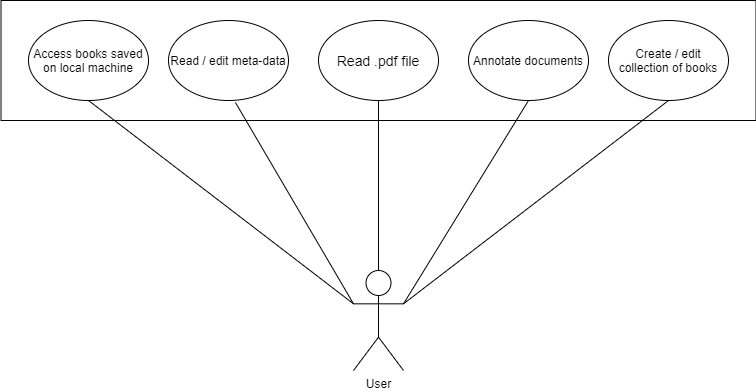
\includegraphics[scale=0.6]{images/User_diag.png}

\newpage
    
\paragraph{} \flushleft
\subsection{Use Cases}
\subsubsection{\texttt{Opening a book}}
\begin{table}[h!]
\begin{tabular}{|l|l|}
\hline
Use case name        & Read book                                                                                                                                       \\ \hline
Scenario             & Open book of .pdf format                                                                                                                        \\ \hline
Triggering event     & User accesses saved file                                                                                                                        \\ \hline
Actors               & User                                                                                                                                            \\ \hline
Related use cases    & View collection                                                                                                                                 \\ \hline
Preconditions        & None                                                                                                                                            \\ \hline
Postconditions       & .pdf file is opened in reader view                                                                                                              \\ \hline
Flow of events       & \begin{tabular}[c]{@{}l@{}}User opens collection or browses explorer\\ User selects a book to read\\ Book is opened in reader view\end{tabular} \\ \hline
Exception Conditions & \begin{tabular}[c]{@{}l@{}}If the user attempts to open unsupported file\\ they will be shown an error message.\\ \\ If book is missing from saved directory,\\ user is prompted to locate it.\end{tabular}                    \\ \hline
\end{tabular}
\end{table}



\subsubsection{\texttt{Adding book to collection}}
\begin{table}[h!]
\begin{tabular}{|l|l|}
\hline
Use case name        & Add book to collection                                                                                                                                                                                                             \\ \hline
Scenario             & Add a book to a collection                                                                                                                                                                                           \\ \hline
Triggering event     & User clicks 'add book' button                                                                                                                                                                          \\ \hline
Actors               & User                                                                                                                                                                                                                 \\ \hline
Related use cases    & View collection                                                                                                                                                                                                      \\ \hline
Preconditions        & Collection already exists                                                                                                                                                                                            \\ \hline
Post conditions       & Collection is updated                                                                                                                                                                                                \\ \hline
Flow of events       & \begin{tabular}[c]{@{}l@{}}User opens collection\\ User clicks add button\\ Book is added to collection\end{tabular}                                                                                                 \\ \hline
Exception Conditions & \begin{tabular}[c]{@{}l@{}}If the user attempts to add an unsupported file\\ they will be shown an error message.\\ \\ If user attempts to add a duplicate file, they \\ will be asked for confirmation\end{tabular} \\ \hline
\end{tabular}
\end{table}

\newpage
\subsubsection{\texttt{Removing a book from a collection}}
\begin{table}[h!]
\begin{tabular}{|l|l|}
\hline
Use case name        & Delete book                                                                                                                                                     \\ \hline
Scenario             & Delete a book from a collection                                                                                                                                 \\ \hline
Triggering event     & User clicks 'remove book' button                                                                                                                                \\ \hline
Actors               & User                                                                                                                                                            \\ \hline
Related use cases    & View collection                                                                                                                                                 \\ \hline
Preconditions        & Collection already exists                                                                                                                                       \\ \hline
Post conditions       & Collection is updated                                                                                                                                           \\ \hline
Flow of events       & \begin{tabular}[c]{@{}l@{}}User opens collection\\ User selects book\\ User clicks remove button\\ Book is removed from collection\end{tabular}                 \\ \hline
Exception Conditions & \begin{tabular}[c]{@{}l@{}}If the book is the only book in the\\ collection, user will be asked if\\ they wish to delete the collection\\ as well.\end{tabular} \\ \hline
\end{tabular}
\end{table}

\subsubsection{\texttt{Creating collections}}
\begin{table}[h!]
\begin{tabular}{|l|l|}
\hline
Use case name        & New collection                                                                                                                                                                                                          \\ \hline
Scenario             & Creating a new collection                                                                                                                                                                                               \\ \hline
Triggering event     & User clicks 'New collection' button                                                                                                                                                                                     \\ \hline
Actors               & User                                                                                                                                                                                                                    \\ \hline
Related use cases    & None                                                                                                                                                                                                                    \\ \hline
Preconditions        & None                                                                                                                                                                                                                    \\ \hline
Postconditions       & Collection is created                                                                                                                                                                                                   \\ \hline
Flow of events       & \begin{tabular}[c]{@{}l@{}}User lands on homescreen \\ User clicks 'New collection' button\\ Name, type etc. are entered\\ Collection is created.\end{tabular}                                                        \\ \hline
Exception Conditions & \begin{tabular}[c]{@{}l@{}}If collection details match a pre-existing\\ collection, user will be asked for confirmation.\\ \\ If details are missing or incomplete, user will\\ be asked for confirmation.\end{tabular} \\ \hline
\end{tabular}
\end{table}

\newpage
\subsubsection{\texttt{Viewing Collections}}
\begin{table}[h!]
\begin{tabular}{|l|l|}
\hline
Use case name        & View collection                                                                                \\ \hline
Scenario             & Browsing existing collections                                                                  \\ \hline
Triggering event     & User clicks on a collection                                                                    \\ \hline
Actors               & User                                                                                           \\ \hline
Related use cases    & Read Book, Add Book, Delete Book, Delete Collection                                            \\ \hline
Preconditions        & Collection already exists                                                                      \\ \hline
Postconditions       & Collection is opened, listing books and options                                                \\ \hline
Flow of events       & \begin{tabular}[c]{@{}l@{}}User lands on homescreen\\ User clicks on a collection\end{tabular} \\ \hline
Exception Conditions & None                                                                                           \\ \hline
\end{tabular}
\end{table}

\subsubsection{\texttt{Deleting Collections}}
\begin{table}[h!]
\begin{tabular}{|l|l|}
\hline
Use case name        & Delete collection                                                                                                                                                                                                        \\ \hline
Scenario             & Deleting existing collections                                                                                                                                                                                            \\ \hline
Triggering event     & User clicks on 'Delete collection' button                                                                                                                                                                                \\ \hline
Actors               & User                                                                                                                                                                                                                     \\ \hline
Related use cases    & View Collection                                                                                                                                                                                                          \\ \hline
Preconditions        & Collection already exists                                                                                                                                                                                                \\ \hline
Postconditions       & Collection is deleted from library                                                                                                                                                                                       \\ \hline
Flow of events       & \begin{tabular}[c]{@{}l@{}}User lands on homescreen\\ User clicks on a collection\\ User clicks on 'delete collection' button\\ Confirmation prompt is presented\\ Upon confirmation, collection is deleted\end{tabular} \\ \hline
Exception Conditions & None                                                                                                                                                                                                                     \\ \hline
\end{tabular}
\end{table}

\newpage
\subsubsection{\texttt{Sorting Books}}
\begin{table}[h!]
\begin{tabular}{|l|l|}
\hline
Use case name        & Sorting Books                                                                                                                                               \\ \hline
Scenario             & Listing books according to filters                                                                                                                          \\ \hline
Triggering event     & User chooses filter from drop-down menu                                                                                                                     \\ \hline
Actors               & User                                                                                                                                                        \\ \hline
Related use cases    & View Collection                                                                                                                                             \\ \hline
Preconditions        & \begin{tabular}[c]{@{}l@{}}Collection already exists\\ \\ More than one book exists in collection\end{tabular}                                              \\ \hline
Postconditions       & Ordering of books is changed                                                                                                                                \\ \hline
Flow of events       & \begin{tabular}[c]{@{}l@{}}User views collection\\ User chooses a filter from drop-down menu\\ Books change order depending on chosen\\ filter\end{tabular} \\ \hline
Exception Conditions & \begin{tabular}[c]{@{}l@{}}If there are less than at least two books\\ in the collection, there is no order to alter.\end{tabular}                          \\ \hline
\end{tabular}
\end{table}

\subsubsection{\texttt{Adding an independent} book}
\begin{table}[h!]
\begin{tabular}{|l|l|}
\hline
Use case name        & Add book                                                                                                                                                                                                                     \\ \hline
Scenario             & Users adds a book independent of collections                                                                                                                                                                                 \\ \hline
Triggering event     & User clicks 'add book' button                                                                                                                                                                                                \\ \hline
Actors               & User                                                                                                                                                                                                                         \\ \hline
Related use cases    & None                                                                                                                                                                                                                         \\ \hline
Preconditions        & None                                                                                                                                                                                                                         \\ \hline
Postconditions       & Book is added to the library                                                                                                                                                                                                 \\ \hline
Flow of events       & \begin{tabular}[c]{@{}l@{}}User lands on homescreen\\ User clicks add book button\\ User browses for book via explorer\\ Book is added\end{tabular}                                                                          \\ \hline
Exception Conditions & \begin{tabular}[c]{@{}l@{}}If the user attempts to add an unsupported\\ file type, they will be shown an error message\\ \\ If the user attempts to add a duplicate file,\\ they will be asked for confirmation\end{tabular} \\ \hline
\end{tabular}
\end{table}

\newpage
\subsubsection{\texttt{Update Metadata}}
\begin{table}[h!]
\begin{tabular}{|l|l|}
\hline
Use case name        & Edit Metadata                                                                                                                                                                                  \\ \hline
Scenario             & User makes changes to a book's metadata                                                                                                                                                        \\ \hline
Triggering event     & User clicks 'Edit info' button                                                                                                                                                                 \\ \hline
Actors               & User                                                                                                                                                                                           \\ \hline
Related use cases    & None                                                                                                                                                                                           \\ \hline
Preconditions        & Book is currently opened                                                                                                                                                                       \\ \hline
Postconditions       & Metadata is updated                                                                                                                                                                            \\ \hline
Flow of events       & \begin{tabular}[c]{@{}l@{}}User opens a book in reader view\\ \\ User clicks 'Edit info' button\\ Required changes are typed in\\ User clicks 'save' button\\ Metadata is updated\end{tabular} \\ \hline
Exception Conditions & \begin{tabular}[c]{@{}l@{}}If information entered has syntax errors,\\ user is shown an error message\end{tabular}                                                                             \\ \hline
\end{tabular}
\end{table}

\section{Class Diagrams}

\subsubsection{Class Diagram for Backend}
\begin{center}
    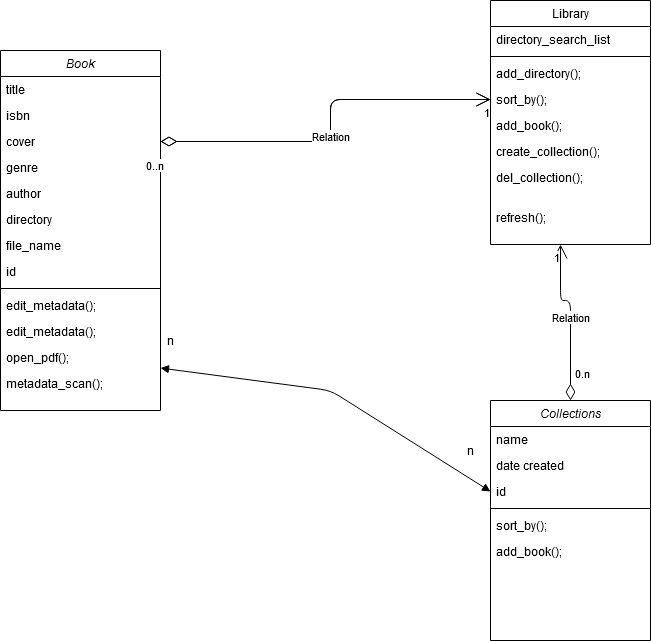
\includegraphics[scale=0.5]{Class Diagram.png}
\end{center}
The above drawn UML diagram shows the relation between the main objects within our software that uses OOP.The PDF reader within the app will utilize \texttt{pdf.js} which is an opensource pdf reader developed by mozilla. The above illustrated diagram pertains to the use cases that are mentioned in Section 2. Since, we are not building the API the UML for the API has been left out.

\section{Sequence Diagrams}
\subsection{Opening a book}
\subsubsection{From explorer:}
\begin{center}
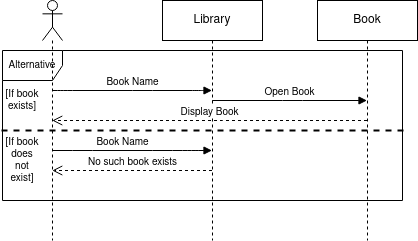
\includegraphics[scale=0.75]{images/seq1a.png}
\end{center}
\subsubsection{From a collection:}
\begin{center}
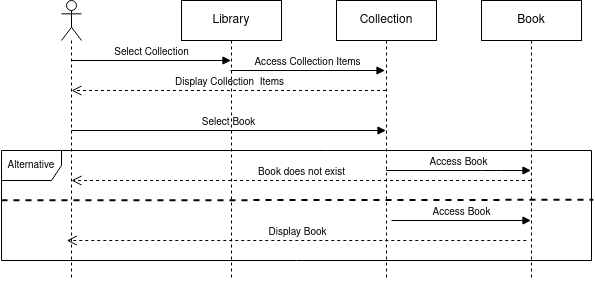
\includegraphics[scale=0.75]{images/seq1b.png}
\end{center}
\newpage
\subsection{Adding a book to collection}
\begin{center}
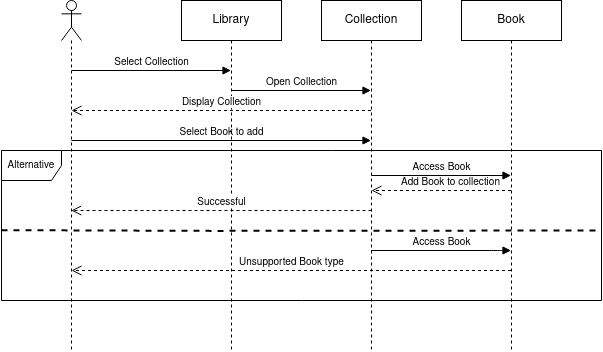
\includegraphics[scale=0.75]{images/seq2.png}
\end{center}
\subsection{Removing a book from collection}
\begin{center}
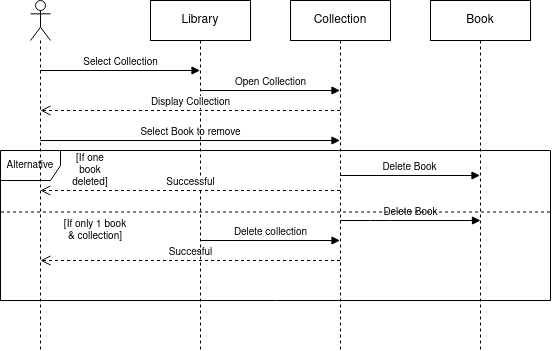
\includegraphics[scale=0.75]{images/seq3.png}
\end{center}
\newpage
\subsection{Creating a collection}
\begin{center}
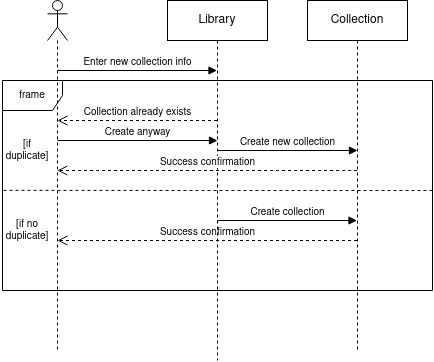
\includegraphics[scale=0.75]{images/seq4.png}
\end{center}
\subsection{Viewing collections}
\begin{center}
    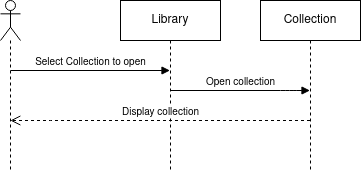
\includegraphics[scale=0.75]{images/seq5.png}
\end{center}
\subsection{Deleting collections}
\begin{center}
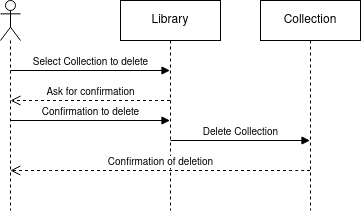
\includegraphics[scale=0.75]{images/seq6.png}    
\end{center}
\subsection{Sorting Books}
\begin{center}
    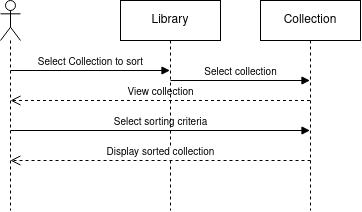
\includegraphics[scale=0.75]{images/seq7.png}
\end{center}
\subsection{Adding an independent book}
\begin{center}
    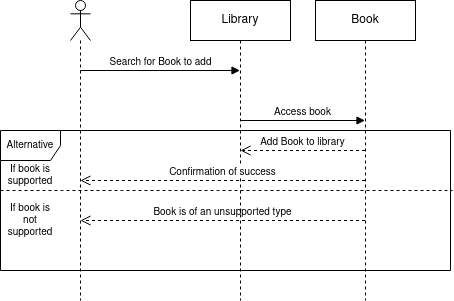
\includegraphics[scale=0.75]{images/seq8.png}
\end{center}
\subsection{Update Metadata}
\begin{center}
    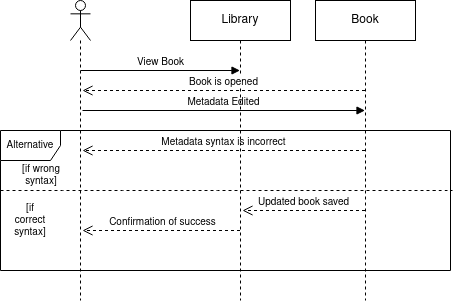
\includegraphics[scale=0.75]{images/seq9.png}
\end{center}
\end{document}